% 固定来源第3页Q24的两幅题图，保留实/虚线、O/H/C/Q等标号。
% 投影 (x,y,z)->(1.5x,.4y+1.5z)，R=SO=1仅为可行构型绘图尺度。
% Q=(-1/2,-sqrt(3)/2,0), C=(1/4,-sqrt(3)/4,0)，H为O到SC垂足。
% 该构型展示原题关系，不在题面增加角度或长度条件。
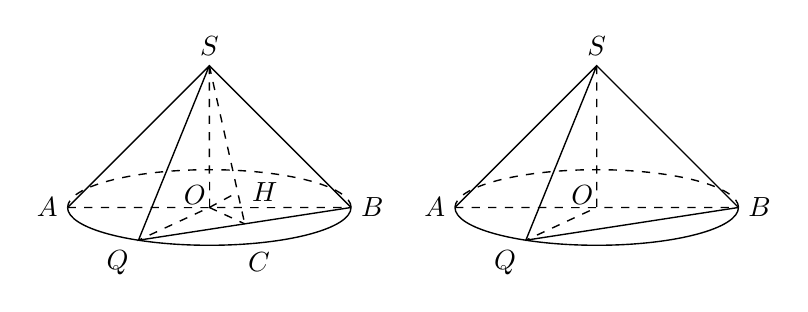
\begin{tikzpicture}[line width=.5pt,scale=1.2]
  \foreach \shift in {0,4.1}{
    \begin{scope}[xshift=\shift cm]
      \coordinate (O) at (0,0);
      \coordinate (S) at (0,1.5);
      \coordinate (A) at (-1.5,0);
      \coordinate (B) at (1.5,0);
      \coordinate (Q) at (-.75,{-.2*sqrt(3)});
      \draw (A) arc[start angle=180,end angle=360,x radius=1.5,y radius=.4];
      \draw[dashed] (B) arc[start angle=0,end angle=180,x radius=1.5,y radius=.4];
      \draw (A)--(S)--(B) (S)--(Q)--(B);
      \draw[dashed] (A)--(B) (S)--(O)--(Q);
      \node[above] at (S) {$S$};
      \node[left] at (A) {$A$};
      \node[right] at (B) {$B$};
      \node[below left] at (Q) {$Q$};
      \node[above left,inner sep=1pt,fill=white] at (O) {$O$};
      \ifdim\shift pt=0pt
        \coordinate (C) at (.375,{-.1*sqrt(3)});
        \coordinate (H) at (.3,{.3-.08*sqrt(3)});
        \draw[dashed] (S)--(C) (O)--(C) (O)--(H);
        \node[below right,inner sep=1pt,yshift=-9pt] at (C) {$C$};
        \node[right,inner sep=2pt,xshift=3pt,fill=white] at (H) {$H$};
      \fi
    \end{scope}
  }
\end{tikzpicture}
